\documentclass[a4paper,12pt]{article}
\usepackage{graphicx}
\usepackage[document]{ragged2e}
\usepackage[utf8]{inputenc}

\title{Printing Techniques}
\author{Rashad Mahmudov}
\date{24 May 2020}

\begin{document}
\maketitle
\section{Introduction}
Printing allows an image to be accurately reproduced a number of times. This process developed to enable mass production of information and images (magazines, posters, fine art pictures), along with the ability to print repeated patterns for fabrics and wallpapers.


Printing techniques include:
\begin{itemize}
\item{Silkscreen printing}
\item{Block printing}
\item{Etching}
\end{itemize}

\section{Silkscreen printing}


Silkscreen printing is sometimes known as the silkscreen process. A print is made using a or acetate placed over a mesh cloth stretched over a heavy frame.

A stencil can be created by carefully cutting out a design from paper and then attaching it to the silkscreen.

\begin{figure}
    \centering
    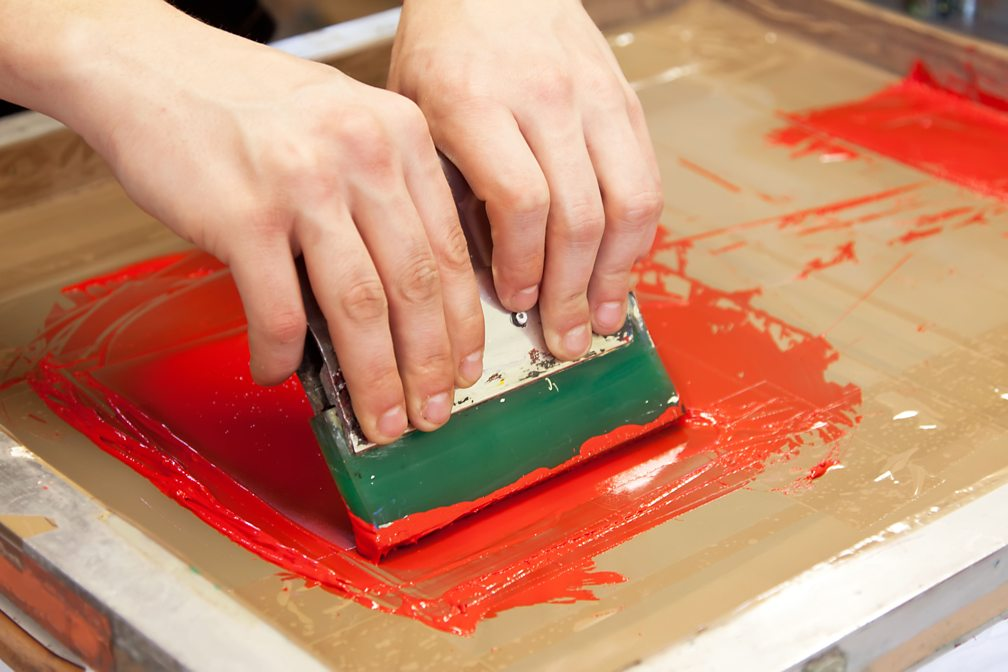
\includegraphics[scale=.7]{img/pic01.jpg}
    \caption{Screen printing technique, Miran Burić}
\end{figure}

If using acetate, you photocopy your image onto an acetate sheet. The screen is coated with a light-sensitive gel and the acetate image is exposed onto
the screen using a ultra-violet light source.
% \newpage
The design is printed by having a squeegee force colour through the pores of the material in the areas that are not blocked out by the stencil.
Silkscreen prints are usually made with acrylic paint that is mixed with a binder to allow the colour to flow easily through the pores and to fix the design.

\subsection*{Uses}
Silkscreen printing is used in many different art and design areas, such as:
\begin{itemize}
\item{Fine art prints}
\item{Posters}
\item{Textiles (Fabric, T-shirts)}
\item{Interiors (Wallpapers, Curtains)}
\end{itemize}
Silkscreen printing is used for small to medium 'runs' of prints. This process can be quite time consuming as it is done manually.


\section{Block (Relief) printing}


Block printing (also called Relief printing) is the process of carving patterns, shapes and designs into a 'block'. The 'block' could be made of wood, acrylic plastic sheet, lino (linoleum) or metal.

\begin{figure}[h!]
    \centering
    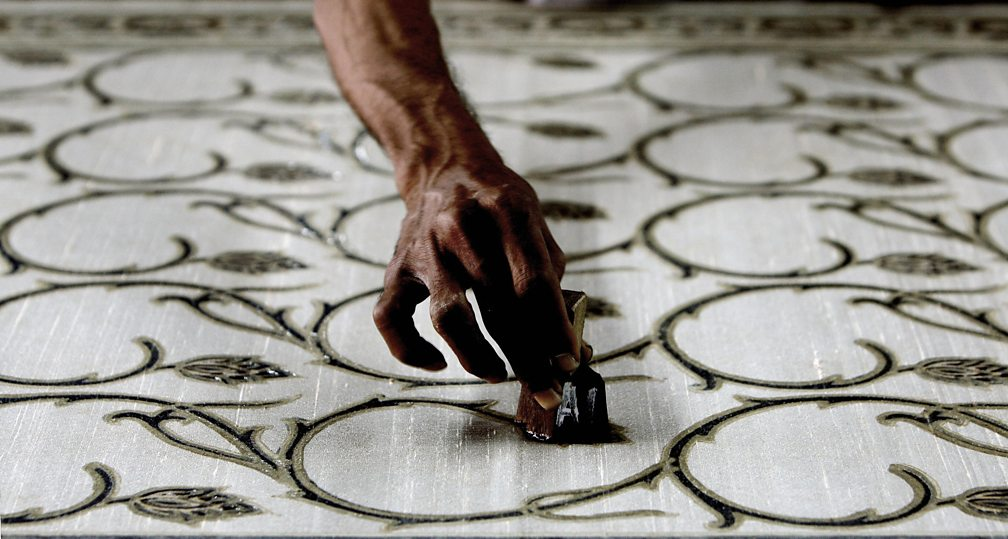
\includegraphics[scale=.7]{img/pic02.jpg}
    \caption{Indian block printing technique, Indranil Mukherjee.}
\end{figure}

Different materials are suited to different results:


\begin{itemize}
\item{Metal or acrylic sheets can produce much finer lines with 'sharper' detail.}
\item{Wood and lino are more suited for bolder images.}
\end{itemize}


The drawback with all of these materials is that each mark you make on the printing sheet will be printed – you cannot afford to make any mistakes.\\ 
Block prints are usually made with oil-based ink.

\begin{enumerate}
  \item Apply the ink to a flat surface, eg an acrylic sheet.
  \item Work the ink with a roller until it becomes 'sticky'.
  \item Roll the ink onto the printing block. This will cover protruding surfaces, leaving recessed areas ink-free.
  \item Use a clean roller or printing press to press the block onto the paper/surface of your final print.
\end{enumerate}

\subsection*{Uses}
Block printing can be used for many purposes, including:
\begin{itemize}
\item{Fine art prints}
\item{Printing lengths of fabrics (look at examples of Indian wood block prints)}
\item{Greetings cards}
\end{itemize}



\section{Etching}
\justifying {Etching is the process of printing produced by ‘etching’ patterns, shapes and designs into the surface of a metal or acrylic plastic plate.
\begin{enumerate}
  \item Scratch your image or design into the surface of the plate.
  \item Apply colour by rolling ink onto the etched surface.
  \item Wipe the surface so that only the ink collected in the in the scratched areas is left.
  \item Carefully place paper on top of the inked sheet.
  \item Use a printing press to apply pressure and lift the image onto your paper.
\end{enumerate}

}

\begin{thebibliography}{3}
\bibitem{Printing Techniques} 
Printing techniques
\\\texttt{https://www.bbc.co.uk/bitesize/guides/z38s6yc/revision/5}

\bibitem{Silkscreen Printing} 
Silkscreen Printing
\\\texttt{https://www.bbc.co.uk/bitesize/guides/z38s6yc/revision/2}

\bibitem{Block (Relief) printing} 
Block (Relief) printing
\\\texttt{https://www.bbc.co.uk/bitesize/guides/z38s6yc/revision/3}

\bibitem{Etching} 
Block (Relief) printing
\\\texttt{https://www.bbc.co.uk/bitesize/guides/z38s6yc/revision/5}

\end{thebibliography}
\end{document}
